\documentclass{article}
\usepackage[margin=1in]{geometry}
\usepackage[nodisplayskipstretch]{setspace}
\usepackage{amsmath, nccmath, bm}
\usepackage{amssymb}
\usepackage{enumitem}
\usepackage{graphicx}
\usepackage{float}
\usepackage{listings}
\usepackage{hyperref}
\usepackage[svgnames]{xcolor}
\usepackage{indentfirst}
%\usepackage{chngcntr}
%\counterwithin{table}{section}
\graphicspath{
{./images}}

%\hypersetup{
%    colorlinks=true,
%    linkcolor=black,
%    filecolor=black,      
%    urlcolor=blue
%    }

\newcommand{\zerodisplayskip}{
	\setlength{\abovedisplayskip}{0pt}%
	\setlength{\belowdisplayskip}{0pt}%
	\setlength{\abovedisplayshortskip}{0pt}%
	\setlength{\belowdisplayshortskip}{0pt}%
	\setlength{\mathindent}{0pt}}
	
\definecolor{vgreen}{RGB}{104,180,104}
\definecolor{vblue}{RGB}{49,49,255}
\definecolor{vorange}{RGB}{255,143,102}

\lstdefinestyle{verilog-style}
{
    language=Verilog,
    basicstyle=\small\ttfamily,
    keywordstyle=\color{vblue},
    identifierstyle=\color{black},
    commentstyle=\color{vgreen},
    numbers=left,
    numberstyle=\tiny\color{black},
    numbersep=10pt,
    tabsize=8,
    moredelim=*[s][\colorIndex]{[}{]},
    literate=*{:}{:}1
}

\lstset{style={verilog-style},showstringspaces=false}

\lstdefinestyle{nocoloring}{
    keywordstyle=\color{black},
    commentstyle=\color{black},
    stringstyle=\color{black}
}

\makeatletter
\newcommand*\@lbracket{[}
\newcommand*\@rbracket{]}
\newcommand*\@colon{:}
\newcommand*\colorIndex{%
    \edef\@temp{\the\lst@token}%
    \ifx\@temp\@lbracket \color{black}%
    \else\ifx\@temp\@rbracket \color{black}%
    \else\ifx\@temp\@colon \color{black}%
    \else \color{vorange}%
    \fi\fi\fi
}
\makeatother

\newcommand{\code}[1]{%
	\colorbox{Gainsboro}{\texttt{#1}}%
}

\title{Lab 3}
\author{Owen Sowatzke}
\date{April 21, 2025}

\begin{document}

	% \offinterlineskip
	% \setlength{\lineskip}{12pt}
	% \zerodisplayskip
	\maketitle
	
	\section{Introduction}
	
	In this lab, we perform design and verification for an ARM 8-bit microprocessor. We start by simulating a SystemVerilog model of the microprocessor in NC verilog. Then, we design 8-bit AND and OR wordslices in Cadence Virtuoso. For each of these wordslices, we create a schematic, symbol, and layout. Then, we incorporate each of our wordslices into the ALU and update its schematic and layout. Similarly, we update the datapath layout with our updated ALU. At each stage of the design, we verify our layouts using DRC and LVS. Finally, we create a netlist from our design and validate its behavior in simulation. 
	
	\section{AND Wordslice}
	
	In this section, we perform design and verification of our AND wordslice. Our wordslice specifically contains 8 \texttt{and2\_1x} gates from the \texttt{muddlib11} library. The resulting schematic is shown in Figure \ref{fig::and2_1x_8_schematic}. Note the vectorized ports and component instances.
	
	\begin{figure}[H]
		\centerline{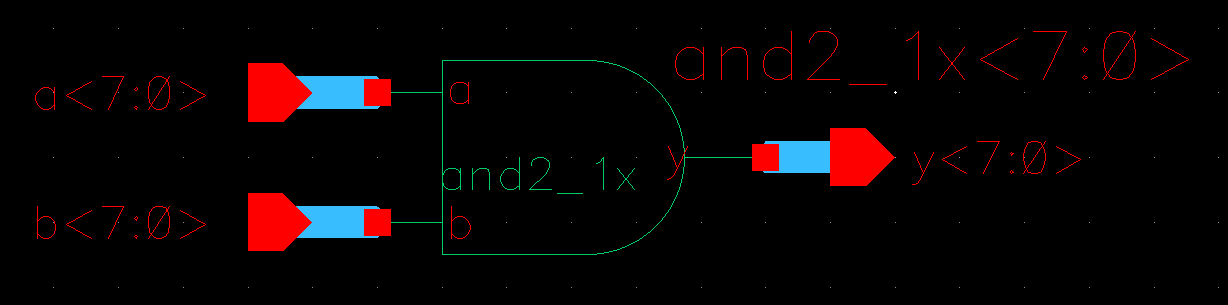
\includegraphics[width=0.5\textwidth]{and2_1x_8_schematic.png}}
		\caption{Schematic for AND Wordslice}
		\label{fig::and2_1x_8_schematic}
	\end{figure}
	
	\noindent Next, we create a symbol for our AND wordslice. For this step, we start with a copy of the \texttt{and2\_1x} symbol and make small incremental updates. Our wordslice symbol with these updates is shown in Figure \ref{fig::and2_1x_8_symbol}. Note that the port names and wire widths have been updated to reflect the vectorized inputs and outputs.
	
	\begin{figure}[H]
		\centerline{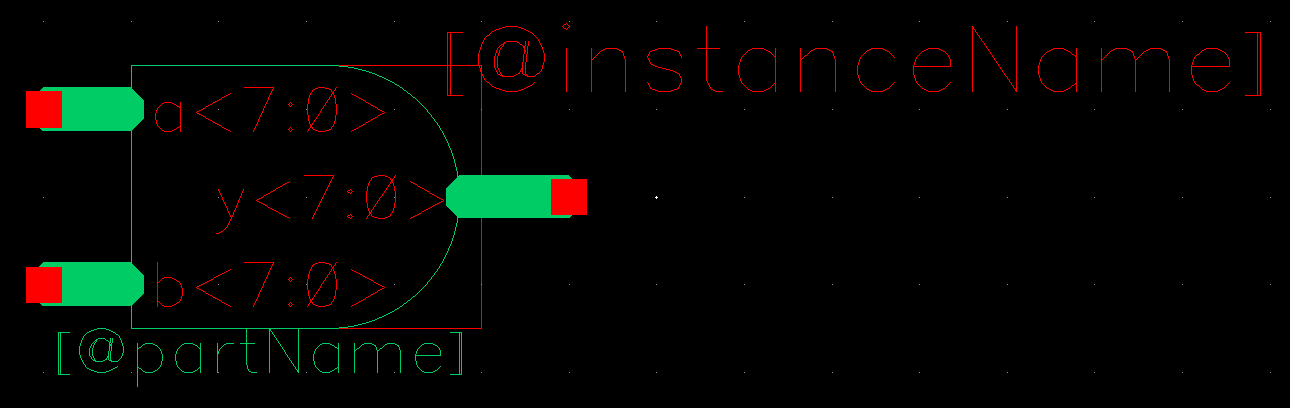
\includegraphics[width=0.5\textwidth]{and2_1x_8_symbol.png}}
		\caption{Symbol for AND Wordslice}
		\label{fig::and2_1x_8_symbol}
	\end{figure}
	
	\noindent Then, we create a layout for our wordslice. To create the layout, we start with a mosiac of AND gates. The resulting layout with different display levels is shown in Figures \ref{fig::and2_1x_8_layout_mosiac_overview} and \ref{fig::and2_1x_8_layout_detailed}.
	
	\begin{figure}[H]
		\centerline{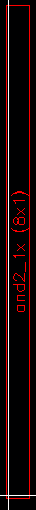
\includegraphics[height=0.8\textwidth, angle=270]{and2_1x_8_layout_mosiac_overview.png}}
		\caption{AND Gate Mosiac Layout Display Level = 0}
		\label{fig::and2_1x_8_layout_mosiac_overview}
	\end{figure}
	
	\begin{figure}[H]
		\centerline{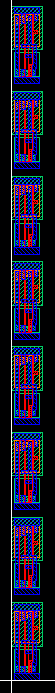
\includegraphics[height=0.8\textwidth, angle=270]{and2_1x_8_layout_detailed.png}}
		\caption{AND Gate Mosiac Layout Display Level = 1}
		\label{fig::and2_1x_8_layout_detailed}
	\end{figure}
	
	\noindent In the layouts, we placed input and output ports for each of the gates. However, in this configuration, virtuoso shorted each element within the vector of pins. These shorts are displayed on an individual AND gates in Figure \ref{fig::and2_1x_8_cell_with_shorts} and in the Annotation Browser in Figure \ref{fig::and2_1x_8_annotation_shorts}. 
	
	\begin{figure}[H]
		\centerline{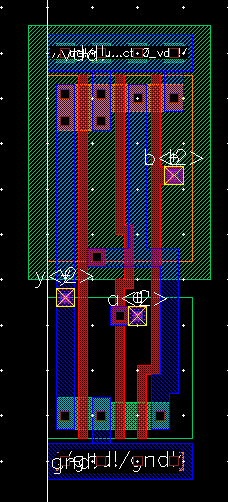
\includegraphics[width=0.2\textwidth]{and2_1x_8_cell_with_shorts.png}}
		\caption{Shorts Marked in the Schematic}
		\label{fig::and2_1x_8_cell_with_shorts}
	\end{figure}
	
	\begin{figure}[H]
		\centerline{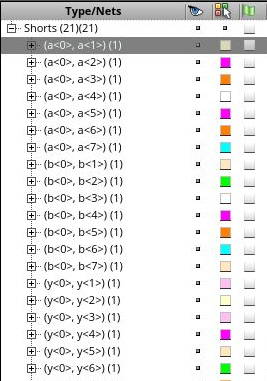
\includegraphics[width=0.35\textwidth]{and2_1x_8_annotation_shorts.png}}
		\caption{Shorts Called Out by the Annotation Browser}
		\label{fig::and2_1x_8_annotation_shorts}
	\end{figure}
	
	\noindent To work around this, I instantiated a single AND gate and then copied it 7 times with $33{\mu}m$ spacing. The resulting schematic at display level = 0 is shown in Figure \ref{fig::and2_1x_8_layout_overview}. Note that the AND gates are now displayed individually at this display level = 0, but the instantiated gates should be identical.
	
	\begin{figure}[H]
		\centerline{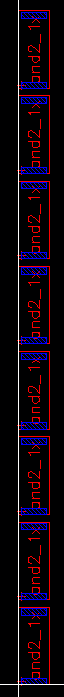
\includegraphics[height=0.8\textwidth, angle=270]{and2_1x_8_layout_overview.png}}
		\caption{AND Wordslice Created without Mosiac at Display Level = 0}
		\label{fig::and2_1x_8_layout_overview}
	\end{figure}
	
	\noindent We also highlight the port placement for a single AND gate, which is shown in Figure \ref{fig::and2_1x_8_single_gate_ports}.
	
	\begin{figure}[H]
		\centerline{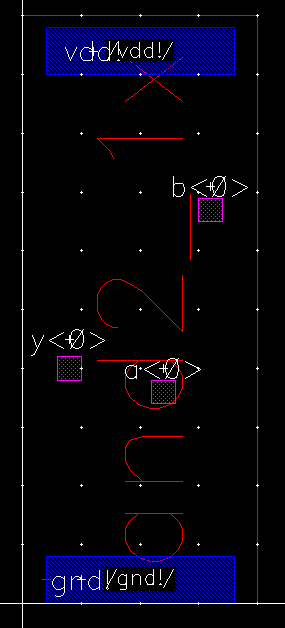
\includegraphics[width=0.25\textwidth]{and2_1x_8_single_gate_ports.png}}
		\caption{Port Placement for a Given AND Gate Instance}
		\label{fig::and2_1x_8_single_gate_ports}
	\end{figure}
	
	\section{NOR Wordslice}
\end{document}